\section{Using Legacy GUI}
\label{sec:GUI}
ENVISIoN is equipped with a graphical user interface to simplify the usage of ENVISIoN. 

\subsection{Start-up}
When the user starts the application through a computer terminal (see chapter \ref{sec: start envision}) a window opens, see figure \ref{fig:GUIStartupUbuntu} for Ubuntu and figure for Windows. The start-up window of ENVISIoN has a sidebar menu to the left with different choices. Each choice has its own content to the right. By default, the ``Dataset loader'', is chosen from start. The other possible choices are ``Parser'' or ``About''. Under ``Active datasets'' the loaded datasets will appear. Each alternative will be explained in their own sections in this chapter. The following figures of the GUI in this chapter will be for Windows but the content is the same for every operative system.

\begin{figure}[H]
    \centering
    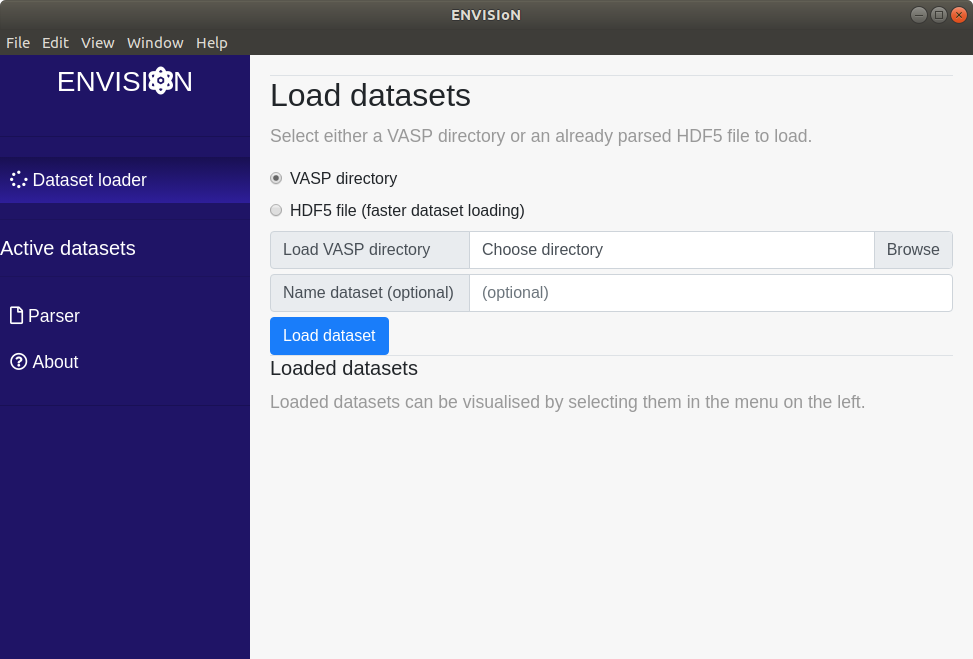
\includegraphics[scale = 0.3]{Images/GUI_start_Ubuntu.png}
    \caption{ENVISIoN start-up window for Linux.}
    \label{fig:GUIStartupUbuntu}
\end{figure}

\begin{figure}[H]
    \centering
    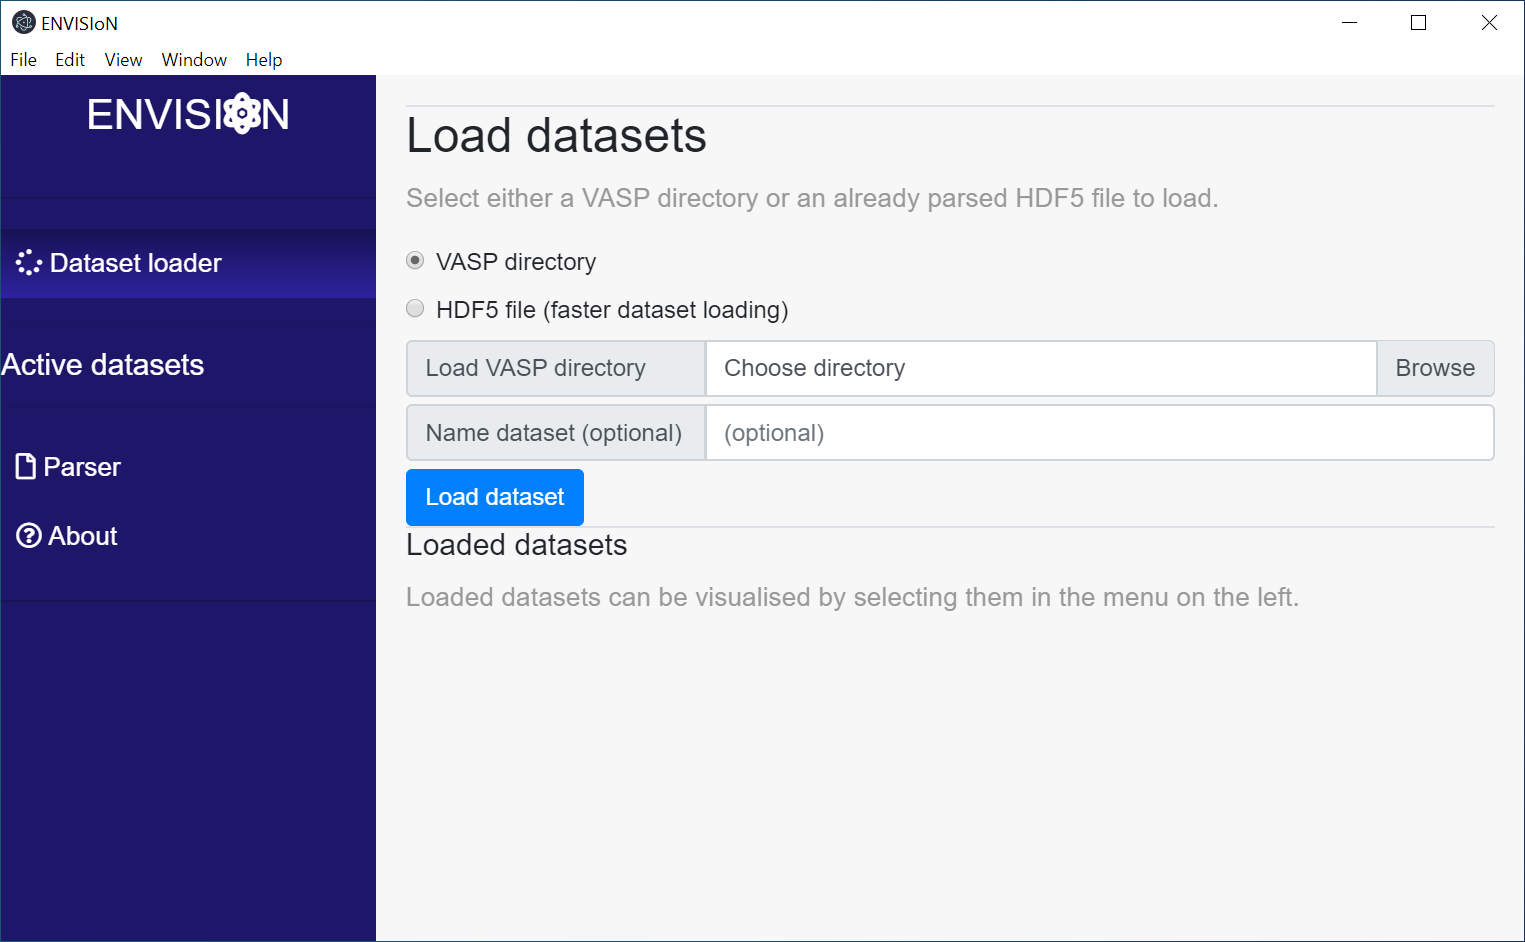
\includegraphics[scale = 0.4]{Images/GUI_start_Windows.png}
    \caption{ENVISIoN start-up window for Windows.}
    \label{fig:GUIStartupUbuntu}
\end{figure}

\subsection{Dataset loader}
In the ``Dataset loader'' a user can select either a VASP file or a HDF5 file to load which then will be visualised. To load a VASP file, the box ``VASP directory'' need to be checked. To load a HDF5 file the box ``HDF5 file'' need to be checked. 

For a quick step-by-step guide, scroll down to section \ref{sec:Dataset step-by-step}.

\subsubsection{Load a VASP file}
For loading a VASP file, the content for the ``Dataset loader'' is shown below in figure \ref{fig:GUIDatasetloaderVASP}.

\begin{figure}[H]
    \centering
    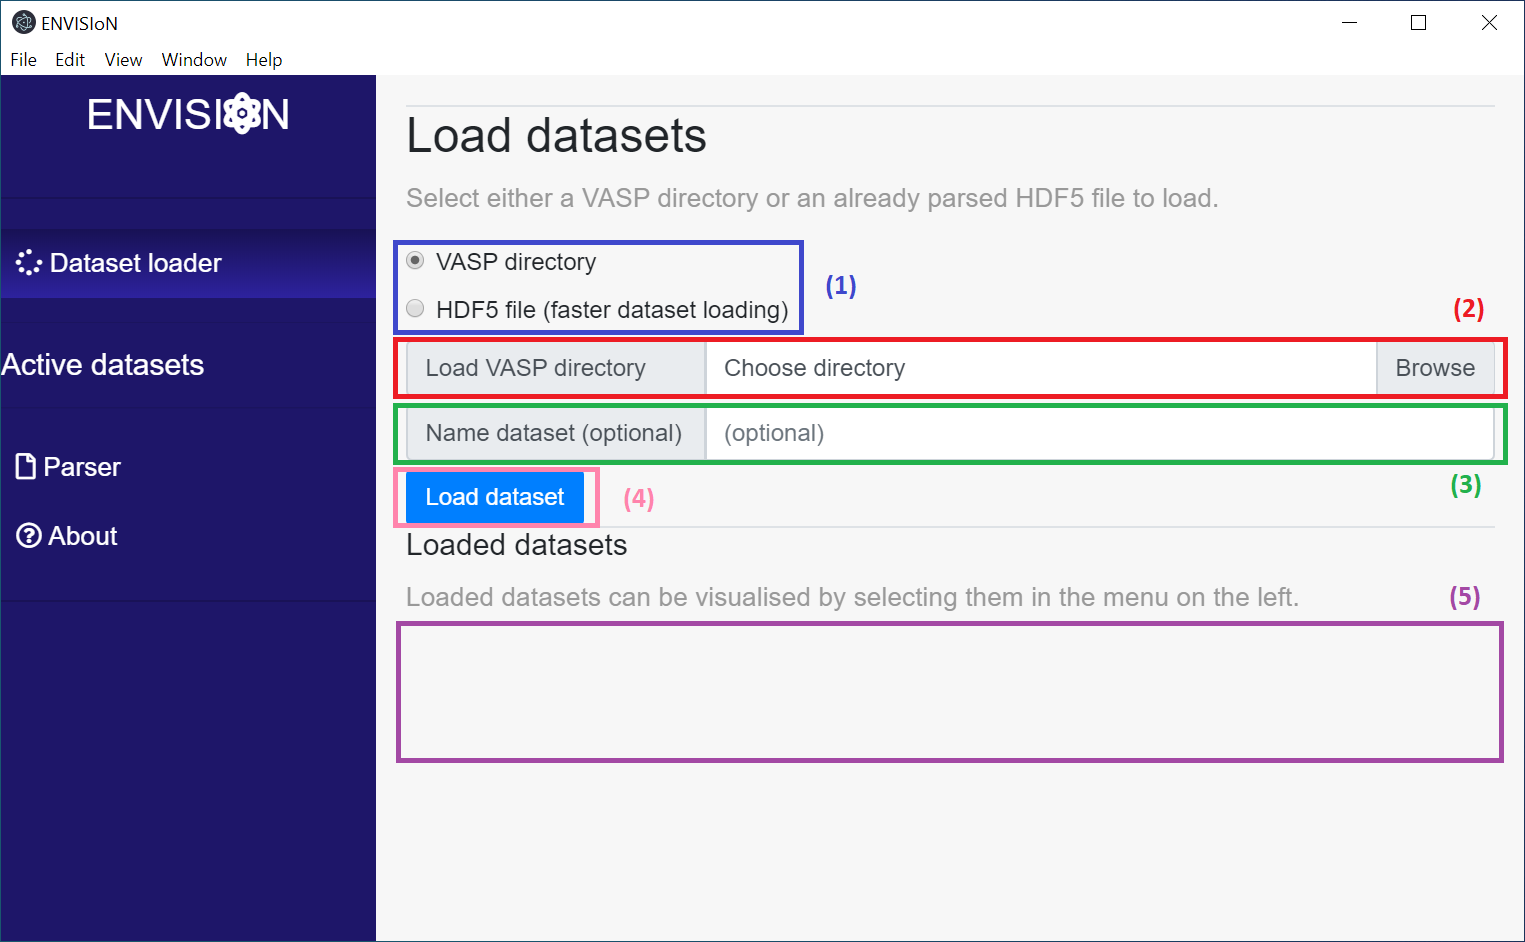
\includegraphics[scale = 0.45]{Images/GUI_Datasetloader_VASP.png}
    \caption{Dataset loader for VASP source.}
    \label{fig:GUIDatasetloaderVASP}
\end{figure}

In the blue box labeled (1) the box ``VASP directory'' need to be checked. In the red box labeled (2) the path to the VASP directory to load is selected. By clicking on ``Browse'' a new window will appear where the user navigates to the VASP directory on the computer and selects it. In the green box labeled (3) the user can write a name for the dataset. This is optional. In the pink box labeled (4) is the ``Load dataset'' button. When pressing this button the dataset will be loaded. The loaded dataset will be displayed in the purple box labeled (5) and in the sidebar menu under ``Active datasets''.

\subsubsection{Load a HDF5 file}
For loading a HDF5 file, the content for the ``Dataset loader'' is shown below in figure \ref{fig:GUIDatasetloaderHDF5}.

\begin{figure}[H]
    \centering
    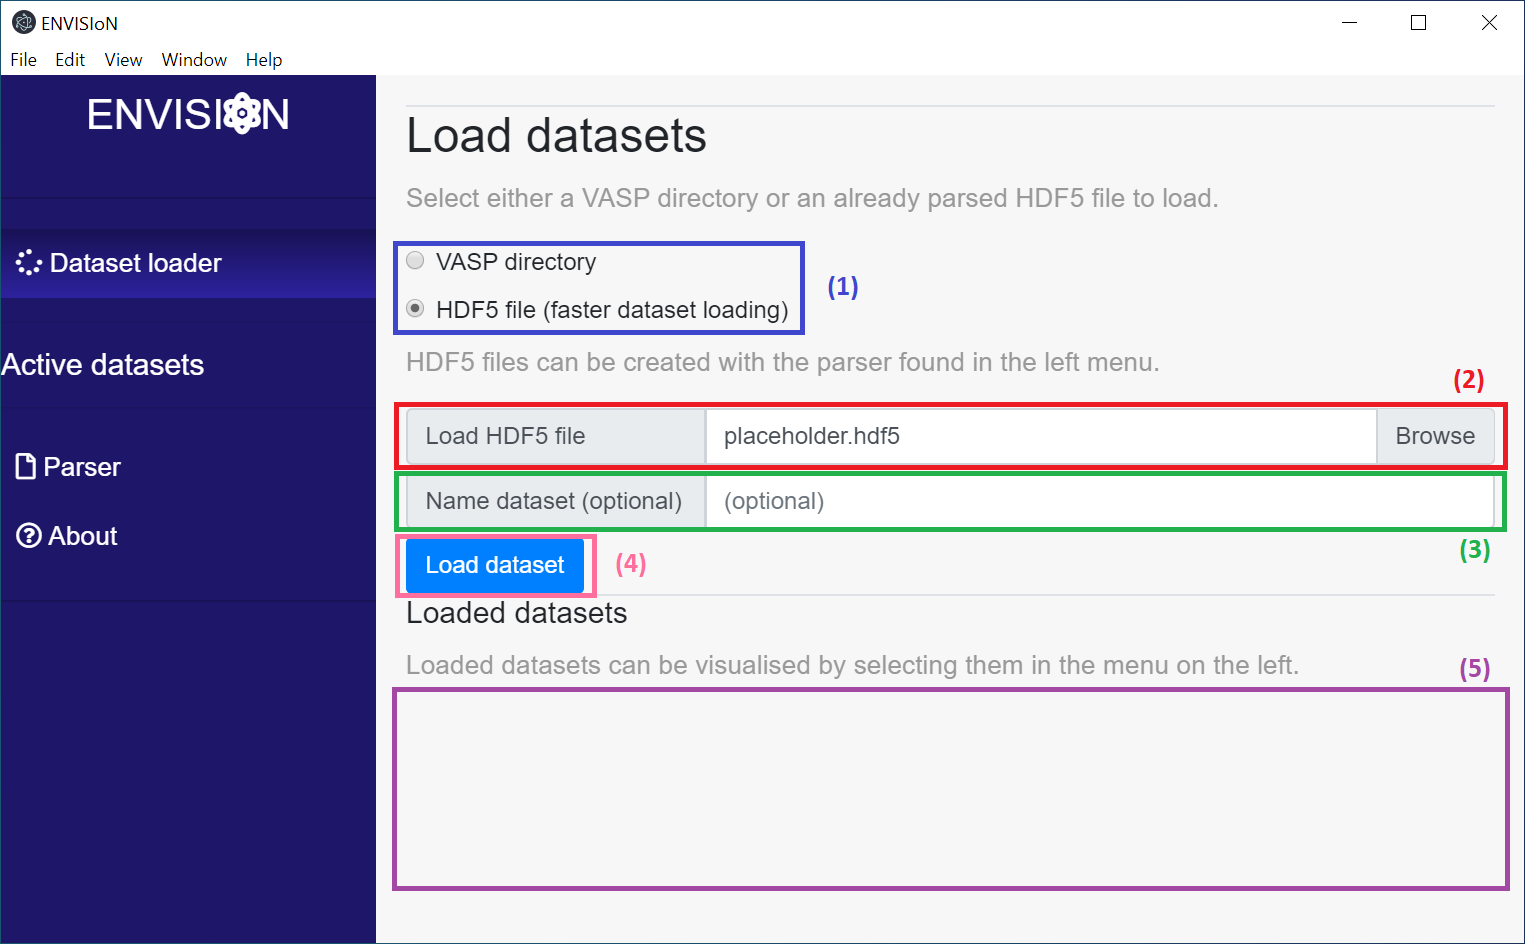
\includegraphics[scale = 0.45]{Images/GUI.Datasetloader_HDF5.png}
    \caption{Dataset loader for HDF5 source.}
    \label{fig:GUIDatasetloaderHDF5}
\end{figure}

In the blue box labeled (1) the box ``HDF5 file'' need to be checked. In the red box labeled (2) the path to the HDF5 file to load is selected. By clicking on ``Browse'' a new window will appear where the user navigates to the HDF5 file on the computer and selects it. In the green box labeled (3) the user can write a name for the dataset. This is optional. In the pink box labeled (4) is the ``Load dataset'' button. When pressing this button the dataset will be loaded. The loaded dataset will be displayed in the purple box labeled (5) and in the sidebar menu under ``Active datasets''.

\subsubsection{Quick Step-by-step guide}
\label{sec:Dataset step-by-step}
To load a VASP-file (referring to figure \ref{fig:GUIDatasetloaderVASP}):
\begin{enumerate}
    \item Check the box ``VASP directory'' in (1).
    \item Choose a VASP directory on your computer by clicking ``Browse'' in (2).
    \item (optional) Name the dataset by writing in (3).
    \item Click ``Load dataset'' in (4).
    \item Now the loaded dataset is showing in (5) and in the sidebar menu under ``Active datasets''.
\end{enumerate}

To load a HDF5 file (referring to figure \ref{fig:GUIDatasetloaderHDF5}):
\begin{enumerate}
    \item Check the box ``HDF5 file'' in (1).
    \item Choose a HDF5 file on your computer by clicking ``Browse'' in (2).
    \item (optional) Name the dataset by writing in (3).
    \item Click ``Load dataset'' in (4).
    \item Now the loaded dataset is showing in (5) and in the sidebar menu under ``Active datasets''.
\end{enumerate}

\subsection{Active datasets}
When a dataset is loaded for visualisation it will appear under ``Active datasets'' in the sidebar menu. 

\subsubsection{Starting the visualisation}
By clicking on one of datasets under ``Active datasets'', new content will show up to the right, see figure \ref{fig:GUIChosevistype} below. In figure \ref{fig:GUIChosevistype} the dataset ``BaSO4\_ORC'' is loaded as an example.

\begin{figure}[H]
    \centering
    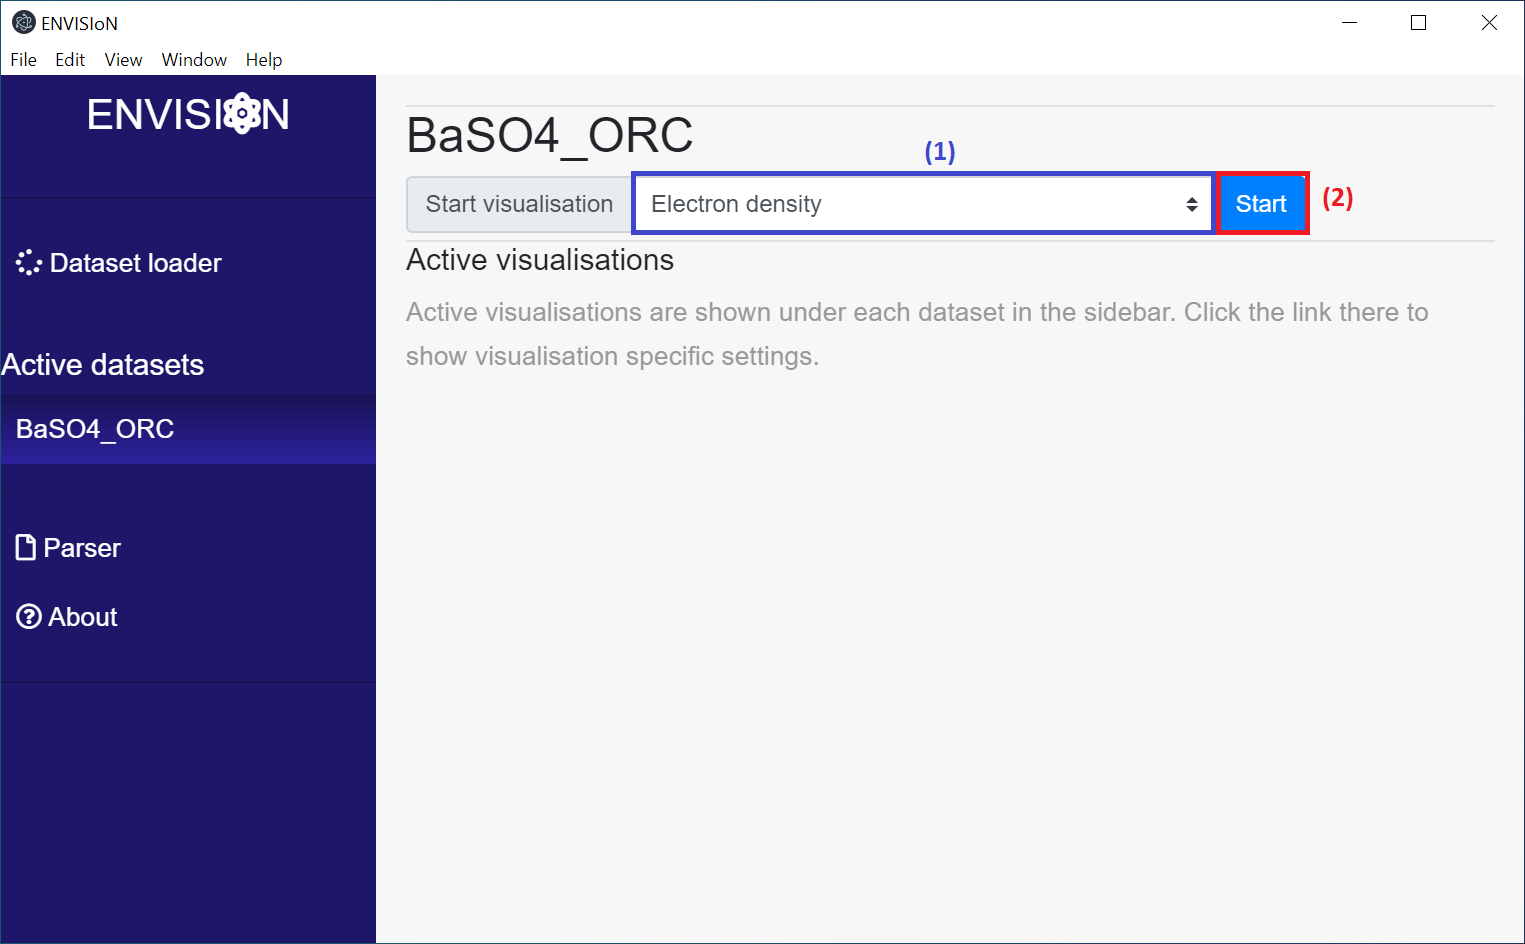
\includegraphics[scale = 0.45]{Images/GUI_Chosevistype.png}
    \caption{Start the visualisation. Here the dataset BaSO4\_ORC is loaded as an example.}
    \label{fig:GUIChosevistype}
\end{figure}

By pressing the area inside the blue box labeled (1) the user can select which visualisation type to visualise from the drop-down menu. The different possible visualisation types are: 

\begin{itemize}
    \item Electron density
    \item Unitcell
    \item Bandstructure 3D
    \item Fermi surface
\end{itemize}

In the red box labeled (2) is the ``Start'' button. When pressing this button the visualisation will start for the chosen visualisation type. The visualisation will appear under the loaded dataset in the sidebar menu. When pressing the visualisation in the sidebar menu new content with visualisation controls will appear to the right. Also the canvas/canvases belonging to the selected visualisation type will pop up next to the GUI.

\subsubsection{Visualisation controls}
When clicking on the ongoing visualisation of a dataset in the sidebar, visualisation controls will appear to the right. These controls are different for different visualisation types. There are only controls for the visualisation types ``Electron density'' and ``Fermi surface''. 

\textbf{Electron density controls}
\newline
If the ongoing visualisation is ``Electron Density'' the controls for interacting with the visualisation are shown in figure \ref{fig:GUICharge} below.

\begin{figure}[H]
    \centering
    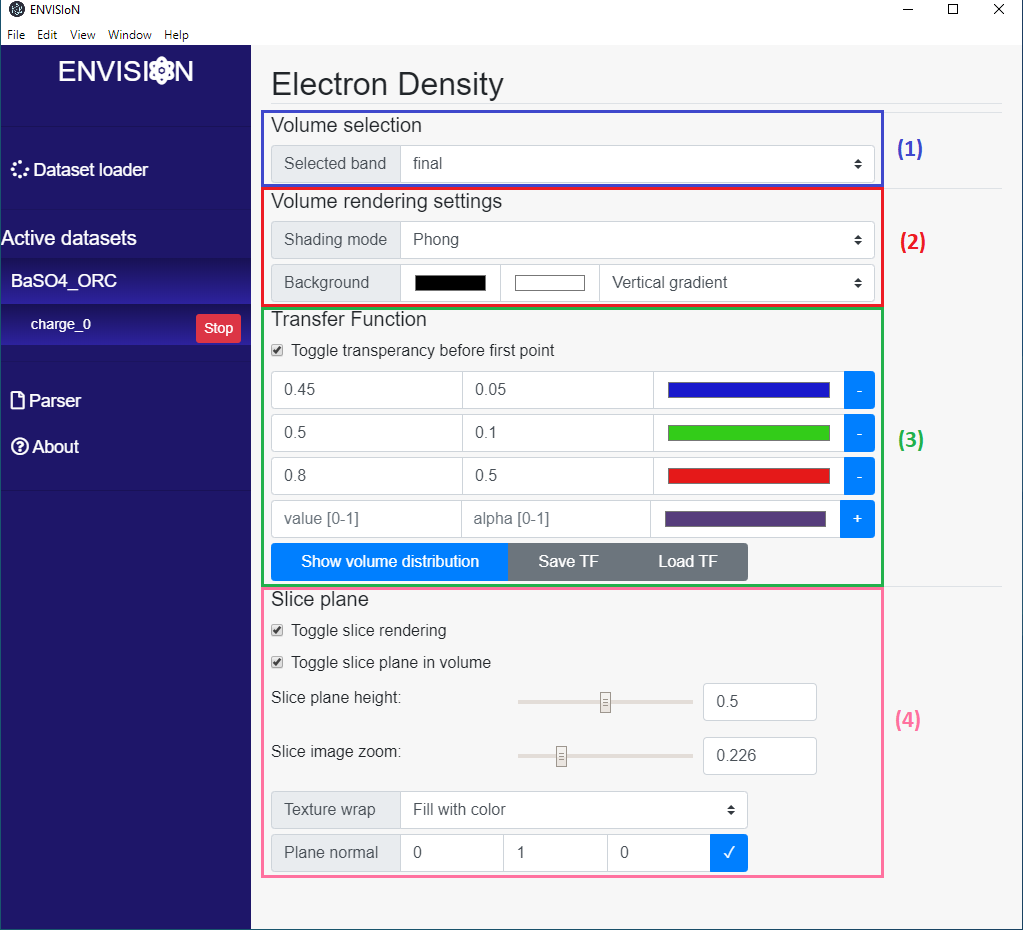
\includegraphics[scale = 0.56]{Images/GUI_Chargecontent.png}
    \caption{The content for the electron density visualisation controls.}
    \label{fig:GUICharge}
\end{figure}

For electron density the user can control the volume selection by selecting band, the volume rendering settings, the transfer function by visualising certain density intervals with different colors and the slice plane to see the electron density in a 2-dimensional plane. In the blue box labeled (1) the user can regulate the volume selection by selecting which band to visualise from a drop-down menu. In the red box labeled (2) the user can select the Shading mode from a drop-down menu and also change the Background color and gradient. In the green box labeled (3) the user can change the transfer function. This is a way to choose different colors for different electron density intervals. The intervals are normalized. The user can also select the blue ``Show volume distribution'' button and then a new diagram will pop up containing information about the volume distribution for the selected dataset. In the pink box labeled (4) the user can configure the slice plan to see a 2-dimensional cross-sectional area of the electron density connected to the 3-dimensional electron density.

\textbf{Fermi surface controls}
\newline
If the ongoing visualisation is ``Fermi surface'' the controls for interacting with the visualisation are shown in figure \ref{fig:GUIFermi} below.

\begin{figure}[H]
    \centering
    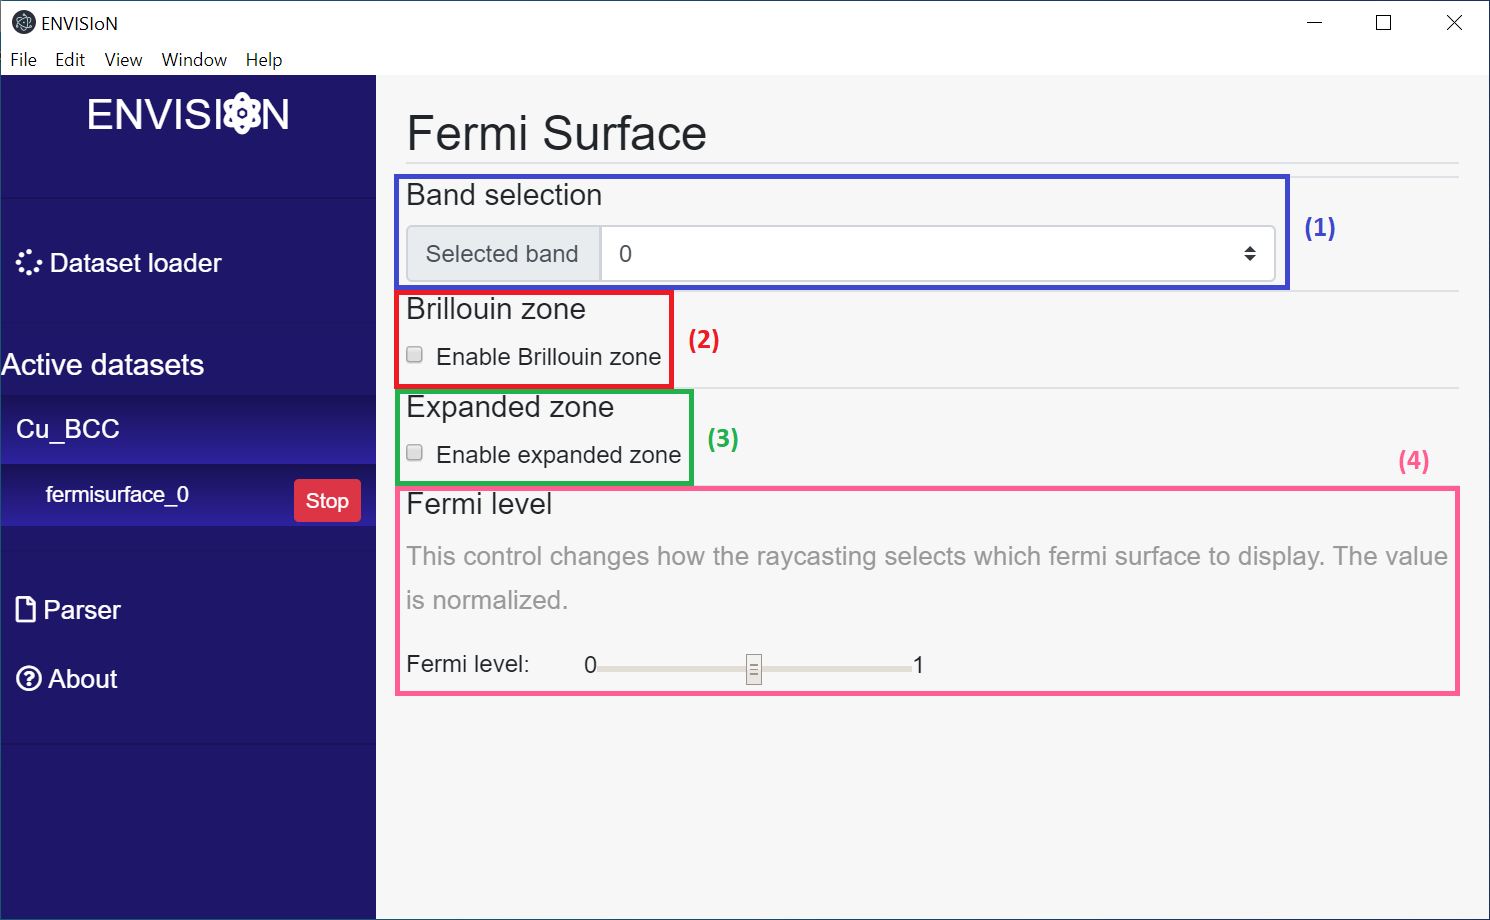
\includegraphics[scale = 0.45]{Images/GUI_Fermicontent.png}
    \caption{The content for the fermi visualisation controls.}
    \label{fig:GUIFermi}
\end{figure}

For fermi surface the user can control which band that should be visualised, enable the Brillouin zone, enable expanded zone and regulate the fermi level. In the blue box labeled (1) the user can select which band to visualise from a drop-down menu. When starting the visualisation the current band will be selected automatically and also the correct fermi level (in the pink box labeled (4)) for each band is set to default. In the red box labeled (2) the user can enable or disable the Brillouin zone by having the checkbox checked or unchecked. In the green box labeled (3) the user can enable or disable expanded zone by having the checkbox checked or unchecked. In the pink box labeled (4) the user can control the fermi level by dragging the slider to the right or to the left. The scale is normalized between 0 and 1.

\subsection{Parser}
If you choose ``Parser'' in the sidebar menu, new content will be exposed to the right, see figure \ref{fig:GUIParser} below. 

\begin{figure}[H]
    \centering
    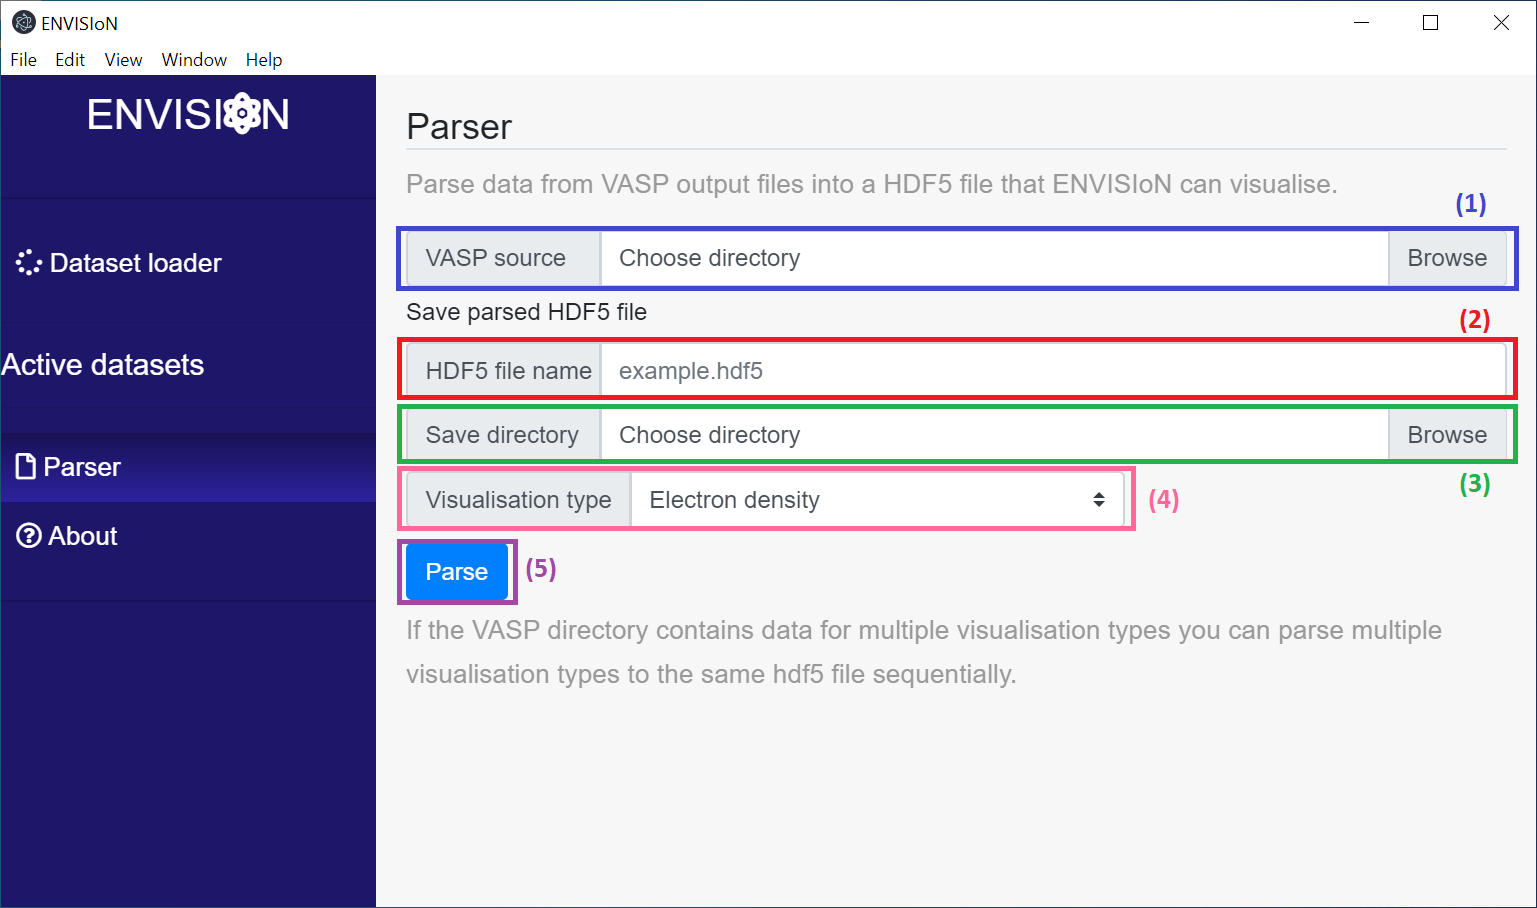
\includegraphics[scale = 0.45]{Images/GUI_Parserstart.png}
    \caption{The content for the parser menu.}
    \label{fig:GUIParser}
\end{figure}

For a quick step-by-step guide, scroll down to section \ref{sec:Parse step-by-step} 

In figure \ref{fig:GUIParser}, in the blue box labeled (1), the path to the directory of VASP files to parse is selected. By clicking on ``Browse'' a new window will appear where the user navigates to the directory of the VASP files on the computer and selects it. In the red box labeled (2) the user writes the name for the new HDF5 file, it needs to end with .hdf5. In the green box labeled (3) the path to the saving directory of the new HDF5 file is selected. When clicking on ``Browse'' a new window will appear where the user navigates to the saving directory and selects it. In the pink box labeled (4) the user can select which visualisation type to parse from a drop-down menu. The possible types to parse are:

\begin{itemize}
    \item Electron density
    \item Bandstructure
    \item Unitcell
    \item Fermi surface
\end{itemize}

In the purple box labeled (5) is the ``Parse'' button. By pressing this button the parser will parse the VASP files and create a HDF5 file in the saving directory. 

\subsubsection{Quick Step-by-step guide}
\label{sec:Parse step-by-step}
Parsing VASP files to a HDF5 file:
\begin{enumerate}
    \item Enter path to VASP directory in (1).
    \item Write name for the HDF5 file in (2).
    \item Enter path to saving directory in (3)
    \item Select type in (4).
    \item Press ``Parse'' in (5).
\end{enumerate}

\subsection{About}
When selecting ``About'' in the sidebar menu there will be new content to the right that contains brief information about ENVISIoN and the project members through the years.

\subsection{If ENVISIoN does not respond or crashes}
If the user have multiple ongoing visualisation or if the user has stopped one visualisation and then want to start another the GUI can stop responding or sometimes even crash. If the GUI falls behind in the number of requests from the user, it will stop responding and a pop up in the GUI will show. The pop up contains the message ``Loading... envision is # requests behind''. See figure \ref{fig:GUINotresponding} below. 

\begin{figure}[H]
    \centering
    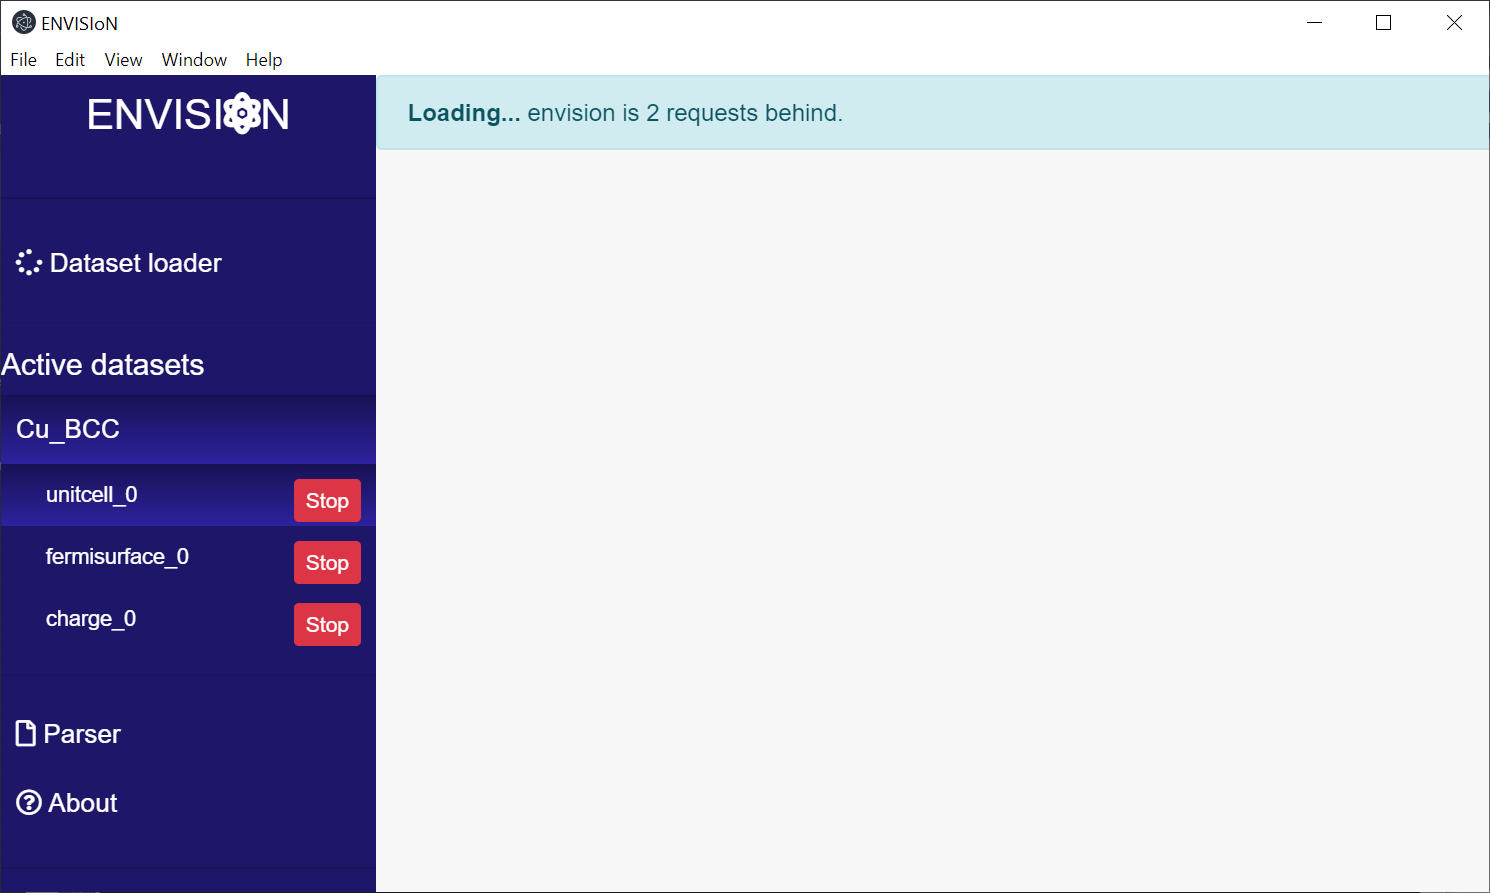
\includegraphics[scale = 0.45]{Images/EnvisionRequestsbehind.png}
    \caption{The pop up when ENVISIoN is a number of requests behind.}
    \label{fig:GUINotresponding}
\end{figure}

To recover from that ENVISIoN is a number of requests behind you can click on ``View'' in the upper menu and then ``Reload'' to reload the GUI. Then you need to start from the beginning and load the dataset once again.

If ENVISIoN is a number of request behind and the user continues to click around in the GUI and tries to load a new dataset or create a new visualisation the GUI will crash. If it does the following message box will pop up, see figure \ref{fig:GUIcrash}.

\begin{figure}[H]
    \centering
    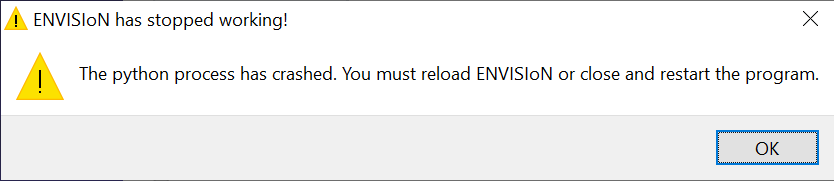
\includegraphics[scale = 0.55]{Images/Envisioncrashed.png}
    \caption{The message box when ENVISIoN crashes.}
    \label{fig:GUIcrash}
\end{figure}

To recover from that ENVISIoN crashes you can either reload the page as mentioned above, or just close the GUI window and restart ENVISIoN.
